\documentclass{beamer}
\usepackage[utf8]{inputenc}

\usetheme{Madrid}
\usecolortheme{default}
\usepackage{amsmath,amssymb,amsfonts,amsthm}
\usepackage{txfonts}
\usepackage{tkz-euclide}
\usepackage{listings}
\usepackage{adjustbox}
\usepackage{array}
\usepackage{tabularx}
\usepackage{gvv} 
\usepackage{lmodern}
\usepackage{circuitikz}
\usepackage{tikz}
\usepackage{graphicx}
\usepackage{gensymb}
\usepackage{amsthm}
\usepackage{mathtools}

\setbeamertemplate{page number in head/foot}[totalframenumber]

\usepackage{tcolorbox}
\tcbuselibrary{minted,breakable,xparse,skins}

\definecolor{bg}{gray}{0.95}
\DeclareTCBListing{mintedbox}{O{}m!O{}}{%
breakable=true,
listing engine=minted,
listing only,
minted language=#2,
minted style=default,
minted options={%
linenos,
gobble=0,
breaklines=true,
breakafter=,,
fontsize=\small,
numbersep=8pt,
#1},
boxsep=0pt,
left skip=0pt,
right skip=0pt,
left=25pt,
right=0pt,
top=3pt,
bottom=3pt,
arc=5pt,
leftrule=0pt,
rightrule=0pt,
bottomrule=2pt,
toprule=2pt,
colback=bg,
colframe=orange!70,
enhanced,
overlay={%
\begin{tcbclipinterior}
\fill[orange!20!white] (frame.south west) rectangle ([xshift=20pt]frame.north west);
\end{tcbclipinterior}},
#3,
}
\lstset{
language=C,
basicstyle=\ttfamily\small,
keywordstyle=\color{blue},
stringstyle=\color{orange},
commentstyle=\color{green!60!black},
numbers=left,
numberstyle=\tiny\color{gray},
breaklines=true,
showstringspaces=false,
}

\title{4.7.40}
\date{September 29, 2025}
\author{EE25BTECH11043 - Nishid Khandagre}

\begin{document}

\frame{\titlepage}

\begin{frame}{Question}
Find the foot of the perpendicular and the perpendicular distance from the point $\myvec{2\\3\\-8}$ to the line $\frac{4-x}{2} = \frac{y}{6} = \frac{1-z}{3}$.
\end{frame}

\begin{frame}{Theoretical Solution}
Given line:
\begin{align}
\frac{4-x}{2}=\frac{y}{6}=\frac{1-z}{3}=t
\end{align}

\begin{align}
x &= 4-2t \\
y &= 6t \\
z &= 1-3t
\end{align}
Line in vector form:
\begin{align}
\myvec{x \\ y \\ z} = \myvec{4 \\ 0 \\ 1} + t \myvec{-2 \\ 6 \\ -3}
\end{align}
\begin{align}
\vec{r} &= \vec{a} + t \vec{m}
\end{align}
\end{frame}

\begin{frame}{Theoretical Solution}
\begin{align}
\vec{a} &= \myvec{4 \\ 0 \\ 1} \\
\vec{m} &= \myvec{-2 \\ 6 \\ -3}
\end{align}
The given point is $\vec{p} = \myvec{2 \\ 3 \\ -8}$
\end{frame}

\begin{frame}{Theoretical Solution}
Let the foot of the perpendicular be $\vec{f}$. Since $\vec{f}$ lies on the line, we can write:
\begin{align}
\vec{f} &= \vec{a} + \alpha\vec{m}
\end{align}
$\myvec{\vec{p} - \vec{f}}$ must be orthogonal to the direction vector of the line $\vec{m}$.\\ \\
Therefore
\begin{align}
\myvec{\vec{p} - \vec{f}}^\top \vec{m} = 0\\
\myvec{\vec{p} - \myvec{\vec{a} + \alpha\vec{m}}}^\top \vec{m} = 0\\
\myvec{\vec{p} - \vec{a} - \alpha\vec{m}}^\top \vec{m} = 0\\
\myvec{\vec{p} - \vec{a}}^\top \vec{m} - \alpha \myvec{\vec{m}^\top \vec{m}} = 0
\end{align}
\end{frame}

\begin{frame}{Theoretical Solution}
\begin{align}
\alpha &= \frac{\myvec{\vec{p}-\vec{a}}^\top \vec{m}}{\vec{m}^\top \vec{m}}
\end{align}
\begin{align}
\vec{p}-\vec{a} &= \myvec{2 \\ 3 \\ -8} - \myvec{4 \\ 0 \\ 1} = \myvec{-2 \\ 3 \\ -9}
\end{align}
\begin{align}
\myvec{\vec{p}-\vec{a}}^\top \vec{m} &= \myvec{-2 & 3 & -9} \myvec{-2 \\ 6 \\ -3} \\
&= (-2)(-2) + (3)(6) + (-9)(-3) \\
&= 4 + 18 + 27 = 49
\end{align}
\end{frame}

\begin{frame}{Theoretical Solution}
\begin{align}
\vec{m}^\top \vec{m} &= (-2)^2 + 6^2 + (-3)^2 \\
&= 4 + 36 + 9 = 49
\end{align}
Therefore
\begin{align}
\alpha &= \frac{49}{49} = 1
\end{align}
foot of the perpendicular $\vec{f}$:
\begin{align}
\vec{f} &= \vec{a} + \alpha\vec{m} \\
&= \myvec{4 \\ 0 \\ 1} + 1 \myvec{-2 \\ 6 \\ -3} \\
&= \myvec{2 \\ 6 \\ -2}
\end{align}
\end{frame}

\begin{frame}{Theoretical Solution}
\begin{align}
\text{Perpendicular Distance} &= \norm{\vec{p}-\vec{f}}
\end{align}
\begin{align}
\vec{p}-\vec{f} &= \myvec{2 \\ 3 \\ -8} - \myvec{2 \\ 6 \\ -2} \\
&=\myvec{0 \\ -3 \\ -6}
\end{align}
\end{frame}

\begin{frame}{Theoretical Solution}
\begin{align}
\norm{\vec{p}-\vec{f}} &= \sqrt{\myvec{\vec{p}-\vec{f}}^\top \myvec{\vec{p}-\vec{f}}} \\
&= \sqrt{0^2 + (-3)^2 + (-6)^2} \\
&= \sqrt{0 + 9 + 36} \\
&= \sqrt{45} \\
&= 3\sqrt{5}
\end{align}
The perpendicular distance is $3\sqrt{5}$.
\end{frame}

\begin{frame}[fragile]
\frametitle{C Code}
\begin{lstlisting}
#include <stdio.h>
#include <math.h>

// Function to find the foot of the perpendicular and the perpendicular distance
// from a point (x0, y0, z0) to a line
// (x - x1)/a = (y - y1)/b = (z - z1)/c
void find_perpendicular_details(
double x0, double y0, double z0, // Point P
double x1, double y1, double z1, // Point on the line L
double a, double b, double c,    // Direction ratios of the line L
double *foot_x, double *foot_y, double *foot_z, // Output: Foot of perpendicular
double *distance // Output: Perpendicular distance
) {
\end{lstlisting}
\end{frame}

\begin{frame}[fragile]
\frametitle{C Code}
\begin{lstlisting}

// Vector PL (P - L)
double PL_x = x0 - x1;
double PL_y = y0 - y1;
double PL_z = z0 - z1;

// Direction vector of the line L (D)
double D_x = a;
double D_y = b;
double D_z = c;

// Calculate projection of PL onto D: t = (PL . D) / ||D||^2
double dot_product = PL_x * D_x + PL_y * D_y + PL_z * D_z;
double magnitude_D_squared = D_x * D_x + D_y * D_y + D_z * D_z;

double t = dot_product / magnitude_D_squared;
\end{lstlisting}
\end{frame}

\begin{frame}[fragile]
\frametitle{C Code}
\begin{lstlisting}
// Foot of the perpendicular F = L + t * D
*foot_x = x1 + t * D_x;
*foot_y = y1 + t * D_y;
*foot_z = z1 + t * D_z;

// Perpendicular vector PF = F - P
double PF_x = *foot_x - x0;
double PF_y = *foot_y - y0;
double PF_z = *foot_z - z0;

// Perpendicular distance = ||PF||
*distance = sqrt(PF_x * PF_x + PF_y * PF_y + PF_z * PF_z);

}
\end{lstlisting}
\end{frame}

\begin{frame}[fragile]
\frametitle{Python Code using C shared output}
\begin{lstlisting}
import ctypes
import numpy as np
import matplotlib.pyplot as plt
from mpl_toolkits.mplot3d import Axes3D

# Load the shared library
lib_perpendicular = ctypes.CDLL("./code7.so")

# Define the argument types and return type for the C function
lib_perpendicular.find_perpendicular_details.argtypes = [
ctypes.c_double, ctypes.c_double, ctypes.c_double,  # P(x0, y0, z0)
ctypes.c_double, ctypes.c_double, ctypes.c_double,  # L(x1, y1, z1)
ctypes.c_double, ctypes.c_double, ctypes.c_double,  # D(a, b, c)
\end{lstlisting}
\end{frame}

\begin{frame}[fragile]
\frametitle{Python Code using C shared output}
\begin{lstlisting}
ctypes.POINTER(ctypes.c_double), # foot_x
ctypes.POINTER(ctypes.c_double), # foot_y
ctypes.POINTER(ctypes.c_double), # foot_z
ctypes.POINTER(ctypes.c_double)  # distance
]
lib_perpendicular.find_perpendicular_details.restype = None

# Given point P
P_x, P_y, P_z = 2.0, 3.0, -8.0

# Given line: (4 - x)/2 = y/6 = (1 - z)/3
# Rewrite in standard form: (x - x1)/a = (y - y1)/b = (z - z1)/c
# (x - 4)/(-2) = (y - 0)/6 = (z - 1)/(-3)
# Point on the line L
L_x, L_y, L_z = 4.0, 0.0, 1.0

# Direction ratios of the line D
D_a, D_b, D_c = -2.0, 6.0, -3.0
\end{lstlisting}
\end{frame}

\begin{frame}[fragile]
\frametitle{Python Code using C shared output}
\begin{lstlisting}
# Create ctypes doubles to hold the results
foot_x_result = ctypes.c_double()
foot_y_result = ctypes.c_double()
foot_z_result = ctypes.c_double()
distance_result = ctypes.c_double()

# Call the C function
lib_perpendicular.find_perpendicular_details(
P_x, P_y, P_z,
L_x, L_y, L_z,
D_a, D_b, D_c,
ctypes.byref(foot_x_result),
ctypes.byref(foot_y_result),
ctypes.byref(foot_z_result),
ctypes.byref(distance_result)
)
\end{lstlisting}
\end{frame}

\begin{frame}[fragile]
\frametitle{Python Code using C shared output}
\begin{lstlisting}
foot_x_found = foot_x_result.value
foot_y_found = foot_y_result.value
foot_z_found = foot_z_result.value
distance_found = distance_result.value

print(f"The foot of the perpendicular is ({foot_x_found:.2f}, {foot_y_found:.2f}, {foot_z_found:.2f})")
print(f"The perpendicular distance is {distance_found:.2f}")

# Plotting
fig = plt.figure(figsize=(10, 8))
ax = fig.add_subplot(111, projection='3d')

# Plot the given point P
ax.scatter(P_x, P_y, P_z, color='black', s=100, label=f'Point P ({P_x},{P_y},{P_z})')
ax.text(P_x, P_y, P_z, f'  P ', color='black')
\end{lstlisting}
\end{frame}

\begin{frame}[fragile]
\frametitle{Python Code using C shared output}
\begin{lstlisting}
# Plot the foot of the perpendicular F
ax.scatter(foot_x_found, foot_y_found, foot_z_found, color='red', s=100, label=f'Foot of Perpendicular F ({foot_x_found:.2f},{foot_y_found:.2f},{foot_z_found:.2f})')
ax.text(foot_x_found, foot_y_found, foot_z_found, f'  F  ', color='red')

# Plot the line
# Parameter t for the line equation
t = np.linspace(-5, 5, 100) # Extend the line for better visualization
line_x = L_x + t * D_a
line_y = L_y + t * D_b
line_z = L_z + t * D_c
ax.plot(line_x, line_y, line_z, color='green', label='Line L')
\end{lstlisting}
\end{frame}

\begin{frame}[fragile]
\frametitle{Python Code using C shared output}
\begin{lstlisting}
# Plot the perpendicular line segment PF
ax.plot([P_x, foot_x_found], [P_y, foot_y_found], [P_z, foot_z_found], color='purple', linestyle='--', label='Perpendicular PF')

ax.set_xlabel('X-axis')
ax.set_ylabel('Y-axis')
ax.set_zlabel('Z-axis')
ax.set_title('Foot of Perpendicular and Perpendicular Distance in 3D')
ax.legend()
ax.grid(True)
plt.savefig("fig1.png")
plt.show()
\end{lstlisting}
\end{frame}


\begin{frame}[fragile]
\frametitle{Python Code (Direct)}
\begin{lstlisting}
import numpy as np
import matplotlib.pyplot as plt
from mpl_toolkits.mplot3d import Axes3D

def line_gen_num(point1, point2, num_points):
    """
    Generates points along a line segment between two 3D points.
    """
    point1 = np.array(point1).flatten()
    point2 = np.array(point2).flatten()
    t = np.linspace(0, 1, num_points)
    points = np.outer(point1, (1-t)) + np.outer(point2, t)
    return points

def plot_3d_line(ax, point1, point2, label="", color="blue", linestyle="-"):
\end{lstlisting}
\end{frame}


\begin{frame}[fragile]
\frametitle{Python Code (Direct)}
\begin{lstlisting}
    """
    Plots a 3D line segment on a given matplotlib axis.
    """
    line_points = line_gen_num(point1, point2, 2)
    ax.plot(line_points[0], line_points[1], line_points[2], color=color, linestyle=linestyle, label=label)

# Given point P
P = np.array([2, 3, -8])

# Given line in symmetric form: (4-x)/2 = y/6 = (1-z)/3
# Rewrite in standard form: (x-4)/(-2) = (y-0)/6 = (z-1)/(-3)
# This means the line passes through point A = (4, 0, 1) and has direction vector d = (-2, 6, -3)
A_line = np.array([4, 0, 1])
d_line = np.array([-2, 6, -3])
\end{lstlisting}
\end{frame}


\begin{frame}[fragile]
\frametitle{Python Code (Direct)}
\begin{lstlisting}
# The foot of the perpendicular M on the line can be represented as:
# M = A_line + t * d_line = (4 - 2t, 6t, 1 - 3t)
# The vector PM is perpendicular to the direction vector d_line
# PM = M - P = (4 - 2t - 2, 6t - 3, 1 - 3t - (-8))
# PM = (2 - 2t, 6t - 3, 9 - 3t)
# The dot product of PM and d_line must be zero: PM . d_line = 0
# (2 - 2t)(-2) + (6t - 3)(6) + (9 - 3t)(-3) = 0
# -4 + 4t + 36t - 18 - 27 + 9t = 0
# 49t - 49 = 0
# 49t = 49 => t = 1
t_val = 1
\end{lstlisting}
\end{frame}

\begin{frame}[fragile]
\frametitle{Python Code (Direct)}
\begin{lstlisting}
# Calculate the coordinates of the foot of the perpendicular M
M = A_line + t_val * d_line
# M = np.array([4 - 2 * t_val, 6 * t_val, 1 - 3 * t_val]) # Alternative calculation
print(f"The foot of the perpendicular is M = ({M[0]}, {M[1]}, {M[2]})")

# Calculate the perpendicular distance from P to the line
perpendicular_distance = np.linalg.norm(P - M)
print(f"The perpendicular distance from P to the line is = {perpendicular_distance:.2f}")

# --- Plotting the 3D scene ---
fig = plt.figure(figsize=(10, 8))
ax = fig.add_subplot(111, projection='3d')
\end{lstlisting}
\end{frame}

\begin{frame}[fragile]
\frametitle{Python Code (Direct)}
\begin{lstlisting}
# Plot the given point P
ax.scatter(P[0], P[1], P[2], color='black', s=100, label=f'Point P({P[0]},{P[1]},{P[2]})')
ax.text(P[0], P[1], P[2] + 0.5, '  P  ', color='black')

# Plot the foot of the perpendicular M
ax.scatter(M[0], M[1], M[2], color='green', s=100, label=f'Foot of Perpendicular M({M[0]},{M[1]},{M[2]})')
ax.text(M[0], M[1], M[2] + 0.5, '  M  ', color='green')

# Plot the line
# We have A_line and M is also on the line. Pick another point using t = 0 (A_line) and t = 2
line_points_for_plot = np.array([
    A_line + 5 * d_line,
    A_line - 5 * d_line
])
\end{lstlisting}
\end{frame}


\begin{frame}[fragile]
\frametitle{Python Code (Direct)}
\begin{lstlisting}
ax.plot(line_points_for_plot[:,0], line_points_for_plot[:,1], line_points_for_plot[:,2], color='blue', label='Line')

# Plot the perpendicular line segment PM
plot_3d_line(ax, P, M, label='Perpendicular PM', color='purple', linestyle='--')

ax.set_xlabel('X')
ax.set_ylabel('Y')
ax.set_zlabel('Z')
ax.set_title('Foot of Perpendicular and Perpendicular Distance')
ax.legend()
ax.grid(True)
plt.tight_layout()
plt.savefig("fig2.png")
plt.show()

print("3D plot saved as fig2.png")
\end{lstlisting}
\end{frame}

\begin{frame}{Plot by Python using shared output from C}
\begin{figure}[H]
\centering
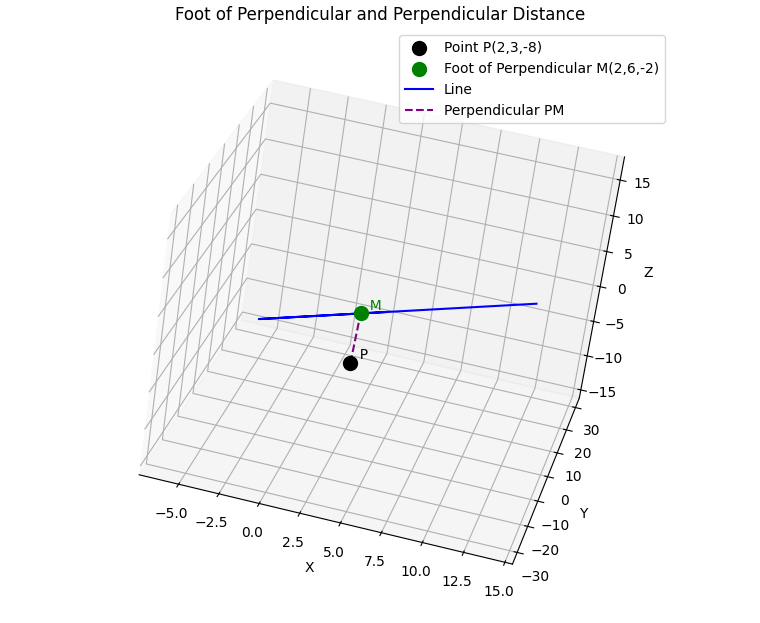
\includegraphics[width=0.8\columnwidth]{../figs/fig1.png}
\caption{}
\label{fig:1}
\end{figure}
\end{frame}
\begin{frame}{Plot by Python only}
\begin{figure}[H]
\centering
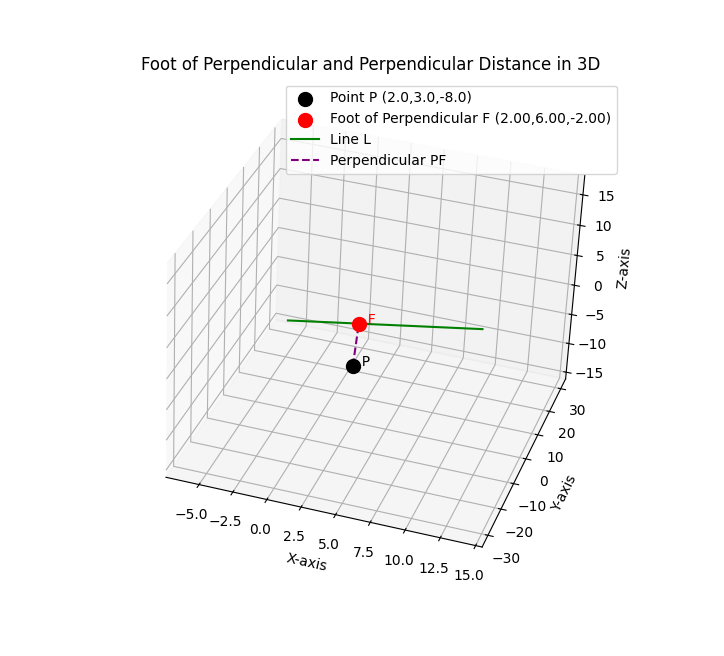
\includegraphics[width=0.8\columnwidth]{../figs/fig2.png}
\caption{}
\label{fig:2}
\end{figure}
\end{frame}

\end{document}
